\chapter{鮮度の視覚化の実装}
\label{chap:implementation}

本章では,第\ref{chap:verification}章で検証した鮮度の表現方法を参考に,実際にブラウザで動作する拡張機能の実装について述べる.

\newpage

\section{システム概要}
\label{sec:imp_system}

本システムは Web ブラウザとして多くのシェアを持つ\footnote{\url{https://gs.statcounter.com/browser-market-share}} Google Chrome の拡張機能での実装を行った.

開発環境には関しては,TypeScript\footnote{\url{https://www.typescriptlang.org/}}, Webpack\footnote{\url{https://webpack.js.org/}} を用いている.

本システムは,Google 検索結果一覧画面に対し,各 Web サイトの公開日を取得することでそれぞれの情報の鮮度を割り出し,外見的な劣化を加える機能を持つ.

第\ref{chap:verification}章で検証した鮮度の表現方法のうち筆者が実装可能かつ実用的だと判断した\ref{subsec:ver-tex-sheet}の表現方法を採用している.

\begin{figure}[htbp]
  \begin{minipage}{0.5\hsize}
    \begin{center}
      \fbox{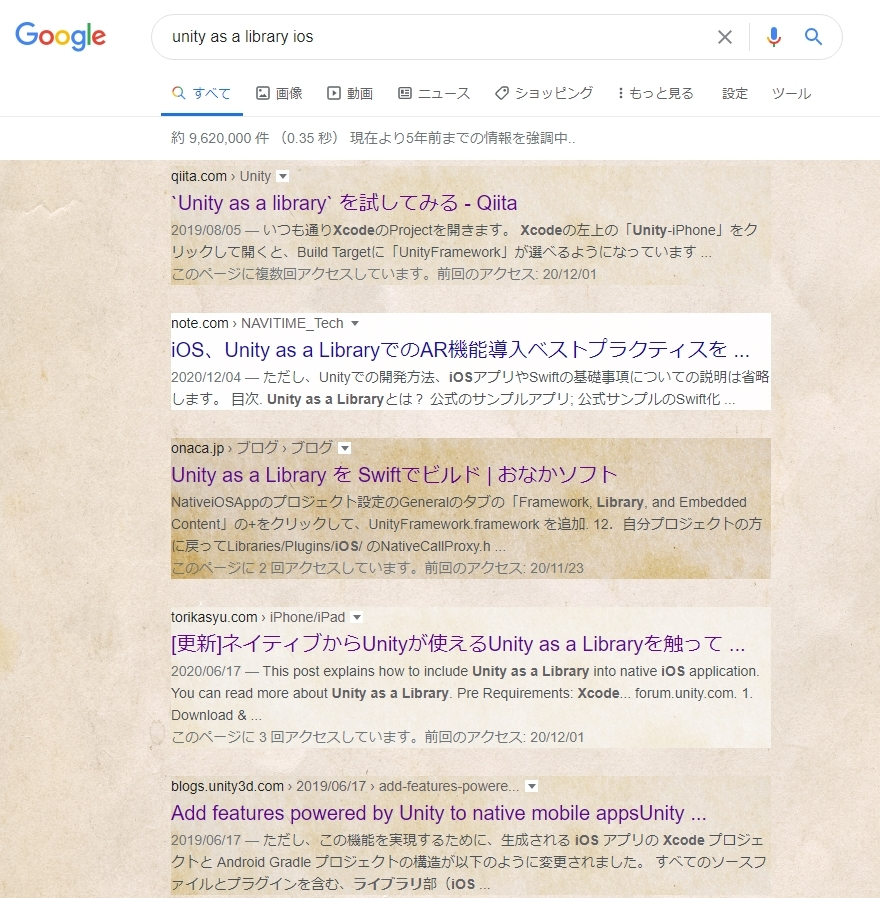
\includegraphics[width=60mm]{images/sample1.jpg}}
    \end{center}
    \caption{運用例1}
  \end{minipage}
  \begin{minipage}{0.5\hsize}
    \begin{center}
      \fbox{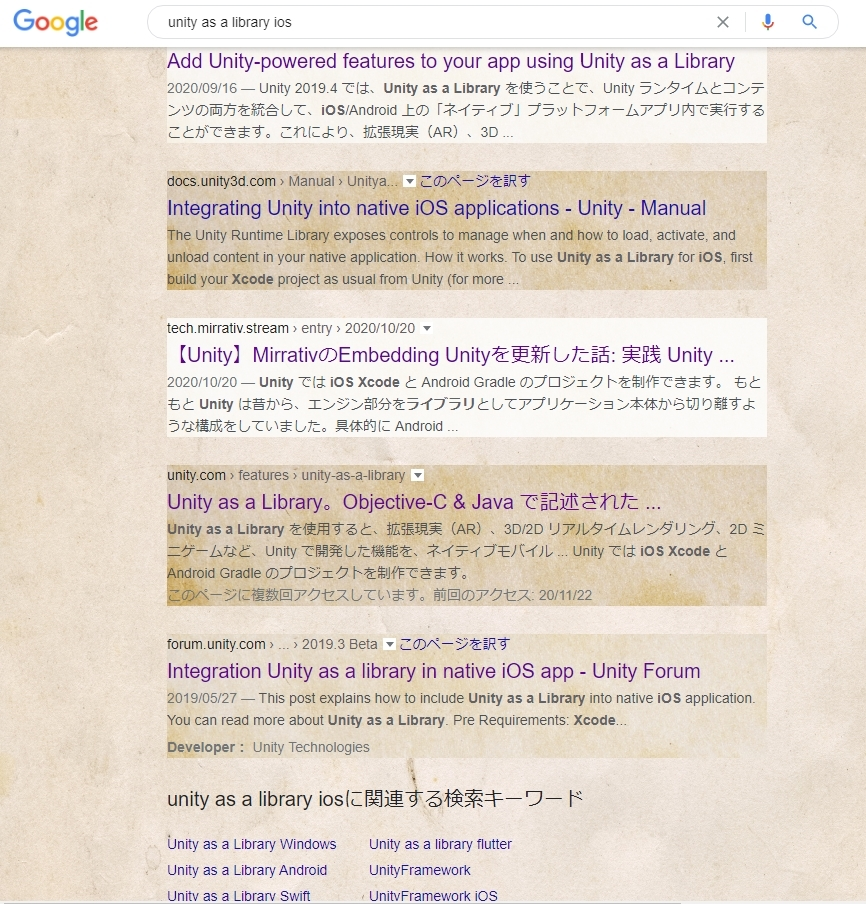
\includegraphics[width=60mm]{images/sample2.jpg}}
    \end{center}
    \caption{運用例2}
  \end{minipage}
\end{figure}

\section{鮮度の算出方法}
\label{sec:imp_calculation}

鮮度(以下 $F$ とする)は0~1の間で表すものとし,1に近ければ近いほど新しいと考える.

また,各情報の公開日を,現在からある年数分までの期間でどの位置に存在するかを0~1の値で表現する(以下 $D$ とする).(例:2018/01/18の情報は,現在(2021/01/24)から 5 年の期間で約 0.6 の位置となる)

以下で示す二つの算出方法をそれぞれ適用し,評価する.

\subsubsection{直線的な算出}

$ F = 1 - D $ の式で鮮度を算出する.シンプルで問題なく利用できる.

\begin{figure}[htbp]
  \begin{center}
    \fbox{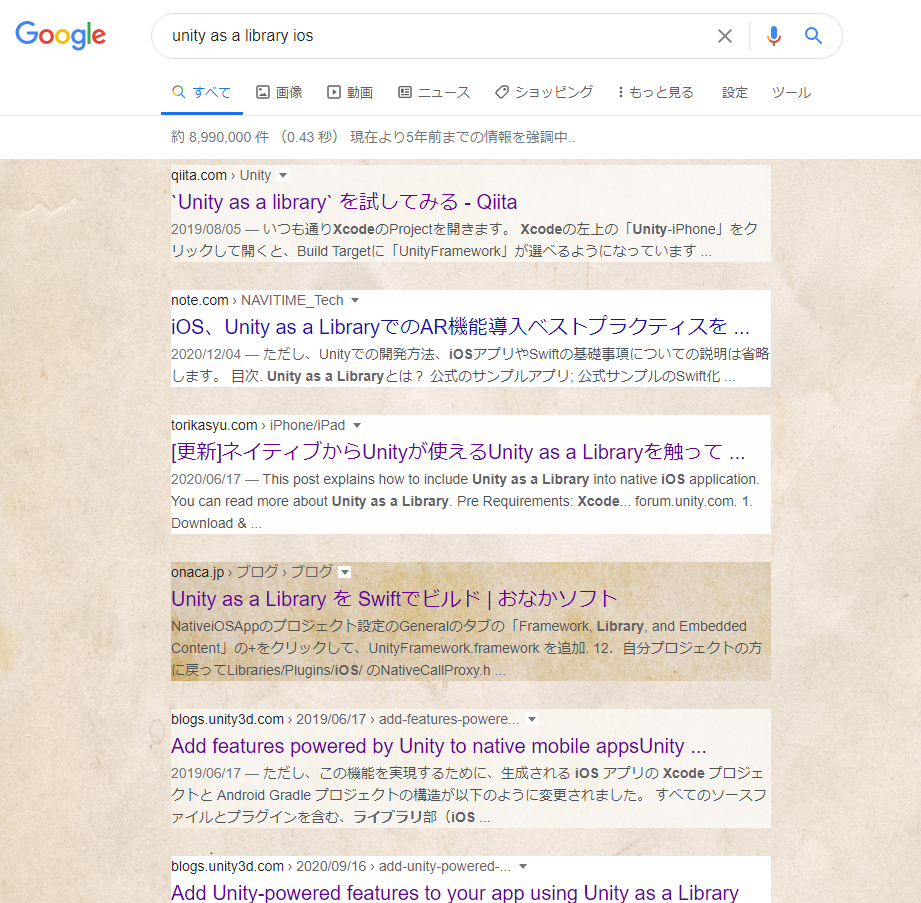
\includegraphics[width=60mm]{images/linear-sample.png}}
  \end{center}
  \caption{$ F = 1 - D $ で算出した例}
\end{figure}

\subsubsection{指数関数的な算出}

$ F =  0.01 ^ D $ の式で鮮度を算出する.少しでも古いものの鮮度が大幅に小さくなるため,より新しい情報を強調することができる.

\begin{figure}[htbp]
  \begin{center}
    \fbox{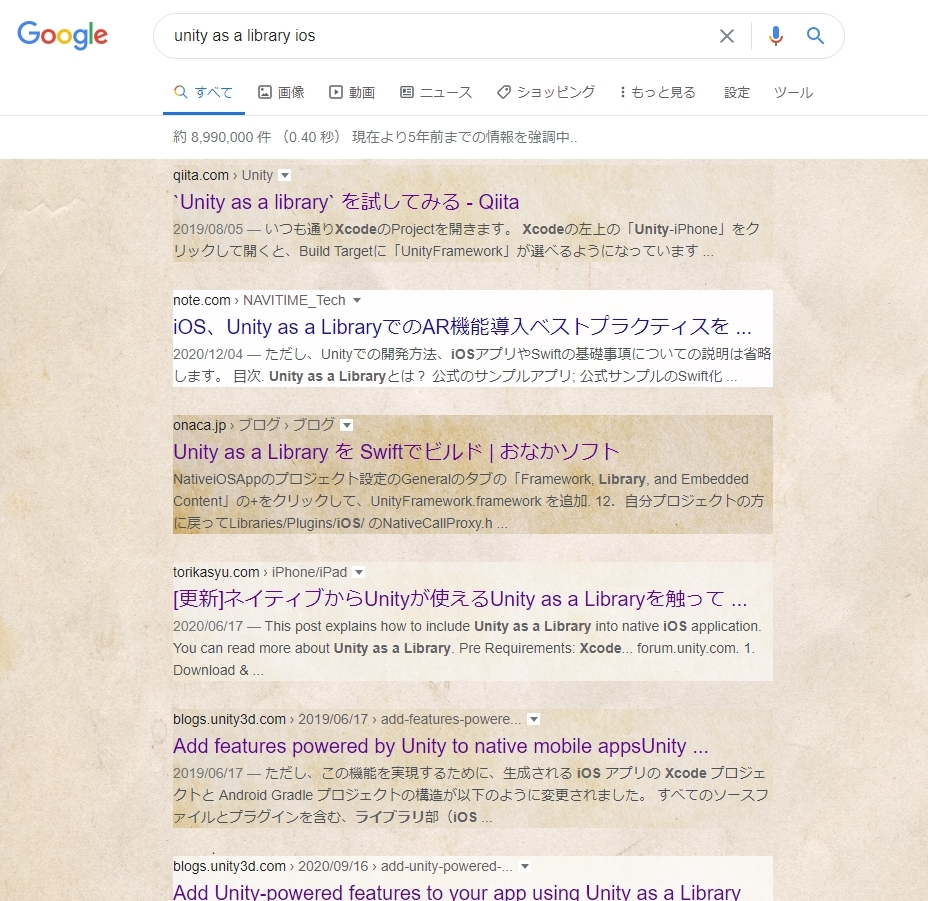
\includegraphics[width=60mm]{images/exponential-sample.png}}
  \end{center}
  \caption{$ F =  0.01 ^ D $ で算出した例}
\end{figure}

\begin{figure}[htbp]
  \begin{minipage}{0.5\hsize}
    \begin{center}
      \fbox{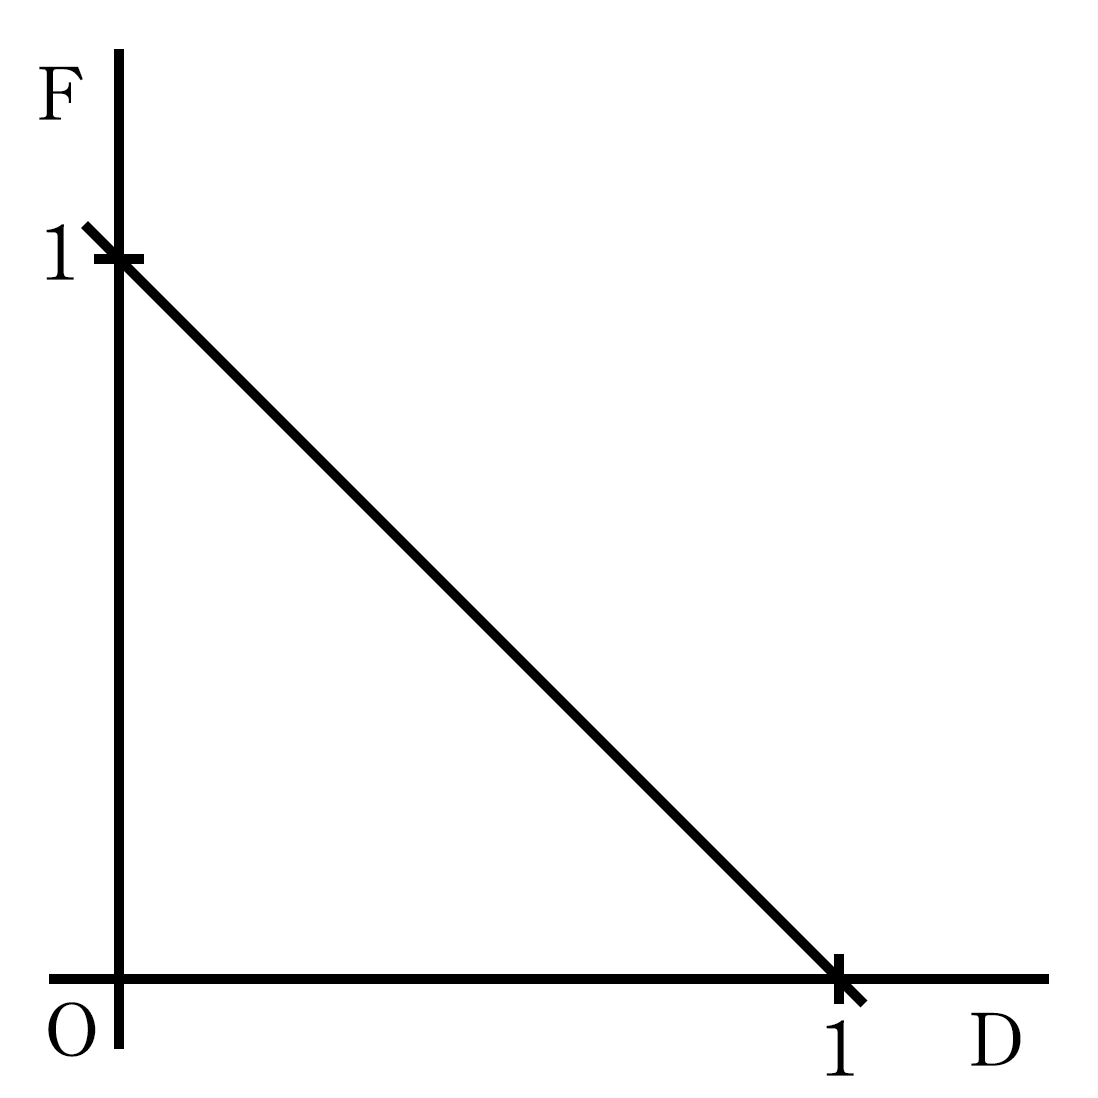
\includegraphics[width=60mm]{images/graph-linear.png}}
    \end{center}
    \caption{直線的な算出方法}
  \end{minipage}
  \begin{minipage}{0.5\hsize}
    \begin{center}
      \fbox{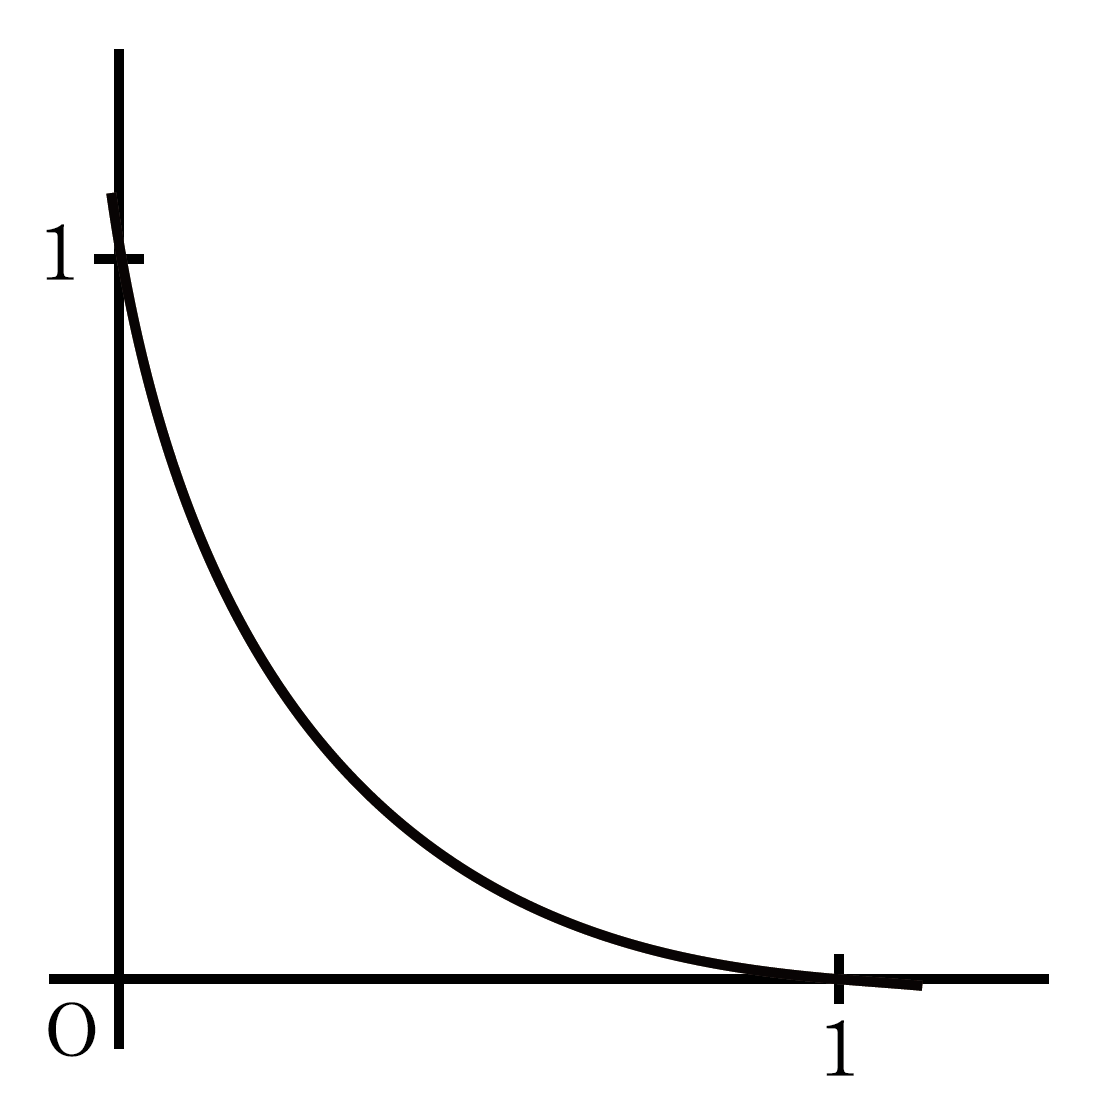
\includegraphics[width=60mm]{images/graph-exponential.png}}
    \end{center}
    \caption{指数関数的な算出方法}
  \end{minipage}
\end{figure}

二つの算出方法を吟味した結果,指数関数的な算出方法の方が直感的に鮮度を感じられたため後者を選択し実装した.
